\section{Aufbau}
\label{sec:Aufbau}
Für die Messung der Reichweite von $\alpha$-Strahlen wird der in \autoref{fig:Aufbau} gezeigte Versuchsaufbau verwendet.
Die benötigten Bauteile sind eine Vakuumpummpe inklusive Druckmessgerät und Ventil, ein Vielkanalanalysator, einen luftdichten Glaszylinder mit Skala zur ABstandsmessung,
den Alphastrahler, einen in \autoref{sec:vorbereitung} beschriebenen Halbleiter-Detektor und einen Vorverstärker.
\begin{figure}
    \centering
    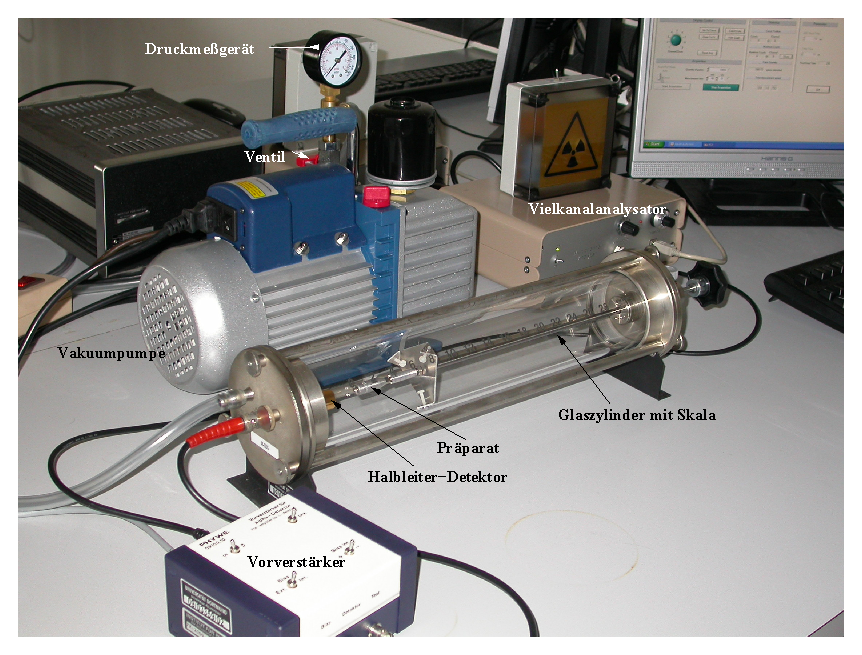
\includegraphics[height = 6cm]{Aufbau.pdf}
    \caption{Aufbau zur Messung der Reichweite von $\alpha$-Strahlen \cite{ap701}.}
    \label{fig:Aufbau}
\end{figure}
Die Bauteile werden ordnungsgemäß angeschlossen und die Messung kann Beginnen.
